\documentclass[11pt, oneside]{article}   	% use "amsart" instead of "article" for AMSLaTeX format
\usepackage{geometry}                		% See geometry.pdf to learn the layout options. There are lots.
\geometry{letterpaper}                   		% ... or a4paper or a5paper or ... 
%\geometry{landscape}                		% Activate for for rotated page geometry
%\usepackage[parfill]{parskip}    		% Activate to begin paragraphs with an empty line rather than an indent
\usepackage{graphicx}				% Use pdf, png, jpg, or eps� with pdflatex; use eps in DVI mode
								% TeX will automatically convert eps --> pdf in pdflatex		
\usepackage{amssymb}

\title{Grafi}
%\author{Fabrizio Demaria}
\date{}							% Activate to display a given date or no date

\begin{document}
\maketitle
\section{Introduzione e definizioni}
Un grafo $G$ \`e una coppia ($V$,$E$), dove $V$ \`e un insieme finito di nodi, chiamati {\bf vertici}, ed $E$ \`e l'insieme degli {\bf archi} di $G$ che definiscono le connessioni tra i vertici. In un {\bf grafo orientato} l'insieme degli archi $E$ \`e una relazione binaria tra i vertici, mentre in un {\bf grafo non orientato} $E$ corrisponde ad un insieme di coppie non ordinate di vertici. In altre parole si dice che se i vertici $u$ e $v$ di un grafo {\em non orientato} sono {\bf adiacenti} (connessi da un arco), la relazione di adiacenza \`e simmetrica. Nel caso di un grafo {\em orientato}, se $u$ \`e adiacente a $v$, non \`e detto che $v$ sia adiacente a $u$.
 Le due tipologie di arco vengono rappresentate come mostrato nella {\em Figura 1}.

%http://www.emeraldinsight.com/content_images/fig/1060210409004.png
\begin{figure}[h]
\begin{center}
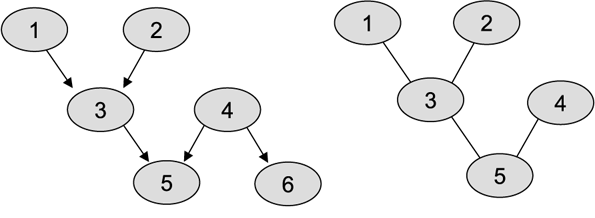
\includegraphics[angle=0,width=0.6\textwidth]{Graphs}
\end{center}
\caption{Grafi orientati (sinistra) e non orientati (destra)}
\end{figure}

Se ($u$,$v$) \`e un arco orientato di un grafo $G$, si dice che l'arco {\bf esce} da $u$ ed {\bf entra} in $v$. Se invece ($u$,$v$) \`e un arco di un grafo non orientato, si dice che l'arco \`e {\bf incidente} nei vertici $u$ e $v$.
In un grafo orientato sono ammessi archi che escono ed entrano nello stesso vertice, denominati {\bf cappi} ({\em self-loops}); in un grafo non orientato i cappi non sono ammessi.

In un grafo non orientato il {\bf grado} di un vertice corrisponde al numero di archi che incidono nel vertice. Per un vertice di un grafo orientato si distinguono un {\bf grado uscente} ed un {\bf grado entrante}, che sono rispettivamente il numero di archi uscenti ed entranti, mentre il {\bf grado} del vertice \`e la somma dei due precedenti.

Un {\bf cammino} \`e una sequenza di vertici di un grafo ottenuta partendo da un vertice iniziale e seguendo determinati archi fino al raggiungimento del nodo finale. La {\bf lunghezza} del cammino \`e il numero di archi attraversati nel cammino. Se esiste un cammino $p$ che presenta come vertice iniziale $u$ e come vertice finale $v$, si dice che $v$ \`e {\bf raggiungibile} da $u$ attraverso $p$. Un cammino \`e definito {\bf semplice} se tutti i vertici di un cammino sono distinti. In un grafo orientato, un cammino il cui nodo di partenza \`e lo stesso del nodo di arrivo \`e detto {\bf ciclo}. Un grafo senza cicli \`e {\bf aciclico}.
\\

Un grafo {\em orientato} \`e {\bf fortemente connesso} se due vertici qualsiasi sono raggiungibili l'uno dell'altro. Un sottoinsieme dei vertici di un grafo per il quale vale la regola sopracitata viene detto {\bf componente fortemente connessa} del grafo. Un grafo orientato pu\`o avere molteplici componenti fortemente connesse, e un grafo \`e fortemente connesso se ha una sola componente fortemente connessa.

Un grafo {\em non orientato} \`e {\bf connesso} se ogni coppia di vertici \`e collegata attraverso un cammino. Un generico grafo non orientato pu\`o essere caratterizzato da molteplici {\bf componenti connesse}, per le quali vale la regola sopracitata. Un grafo non orientato \`e connesso di per s\'e se presenta una sola componente connessa.

\begin{figure}[h]
\begin{center}
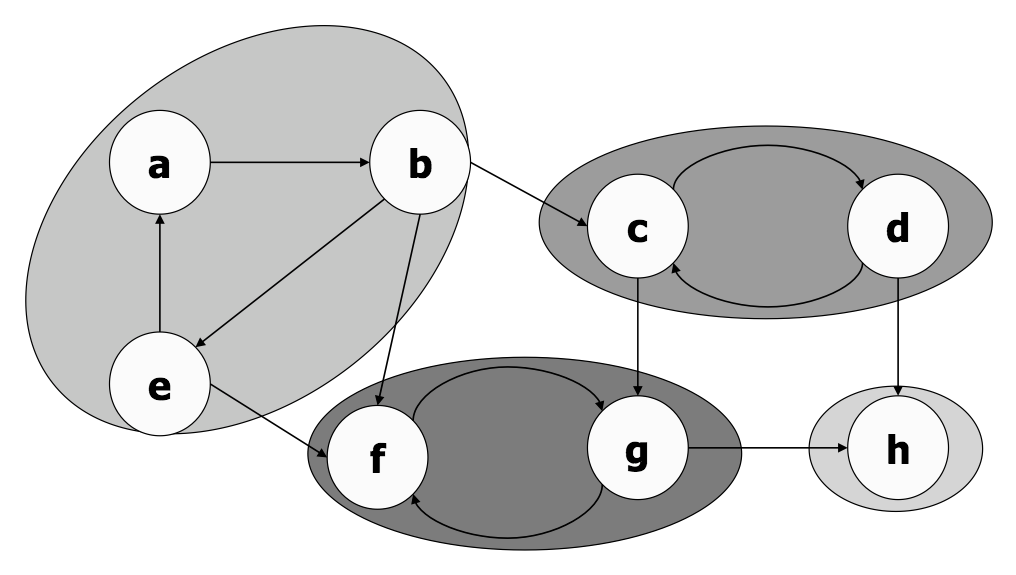
\includegraphics[angle=0,width=0.6\textwidth]{Connected}
\end{center}
\caption{Grafo orientato. I vari insiemi di vertici corrispondono alle componenti fortemente connesse del grafo}
\end{figure}

Ad ogni arco di un generico grafo pu\`o essere associato un indice che ne indica il {\bf peso} (o {\bf costo}). In questo caso si parla di {\bf grafo pesato}.

Infine, un grafo si dice {\bf sparso} quando il numero di archi $|E|$ \`e molto pi\`u piccolo di $|V|^2$. Un grafo \`e invece {\bf denso} se $|E|$ \`e prossimo al valore $|V|^2$.
\\ 

Sulla base delle definizioni precedentemente riportate \`e possibile definire alcuni tipologie specifiche di grafo. Un {\bf grafo completo} \`e un grafo non orientato in cui ogni coppia di vertici \`e adiacente. Un grafo aciclico e non orientato \`e una {\bf foresta}. Un grafo aciclico, non orientato e connesso \`e un {\bf albero} (senza radice). In quest'ultimo caso, ogni coppia di vertici \`e connessa da un singolo cammino semplice, e la rimozione di un qualsiasi arco comporta la disconnessione del grafo (generando una foresta); inoltre, l'aggiunta di un arco  tra due vertici qualsiasi introduce un ciclo facendo si che il grafo non sia pi\`u un albero.

\begin{figure}[h]
\begin{center}
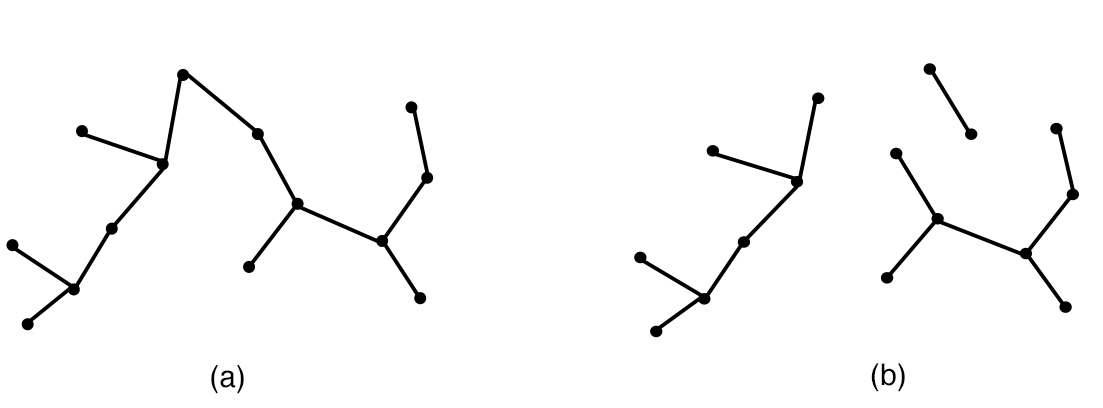
\includegraphics[angle=0,width=0.75\textwidth]{trees}
\end{center}
\caption{(a) Un albero libero; (b) Una foresta }
\end{figure}


Se in un albero come appena descritto viene identificato un {\bf nodo radice}, si possono instaurare tutte le regole di parentela tra nodi. A tal proposito si rimanda al paragrafo introduttivo del capitolo inerente gli alberi per una pi\`u approfondita trattazione.

\section{Rappresentazioni dei grafi}
Un grafo \`e l'ideale per modellare numerose tipologie di problemi, per la soluzione dei quali \`e possibile adottare un determinato algoritmo. In generale, tutti gli algoritmi sui grafi sono basati su tecniche di ricerca in un grafo; effettuare ricerche in un grafo significa seguire gli archi del grafo per visitarne tutti i nodi ed estrapolare dall'operazione alcune informazioni.

In questo contesto, la rappresentazione dei grafi in memoria risulta essere un concetto chiave. In questo capitolo vengono proposti i due metodi standard per la memorizzazione di un grafo: la {\em rappresentazione con liste di adiecanza} e la {\em rappresentazione con matrici di adiacenza}.

\subsection{Rappresentazione con liste di adiacenza}
Questo metodo fa uso di un array $A$ di $|V|$ liste, una per ogni vertice dell'insieme $V$. Per ogni nodo $u$ del grafo, la lista $A[u]$ contiene tutti i vertici $v$ tali per cui esiste un arco $(u,v) \in E$ (cio\`e tutti i vertici adiacenti a $u$).

Se il grafo $G$ considerato \`e orientato, la somma delle lunghezze di tutte le liste di adiacenza \`e esattamente $|E|$, mentre se il grafo non \`e orientato la somma corrisponde a $2|E|$, in quanto per ogni arco non orientato $(u,v)$, $u$ appartiene alla lista di adiacenza di $v$ e viceversa.

\begin{figure}[h]
\begin{center}
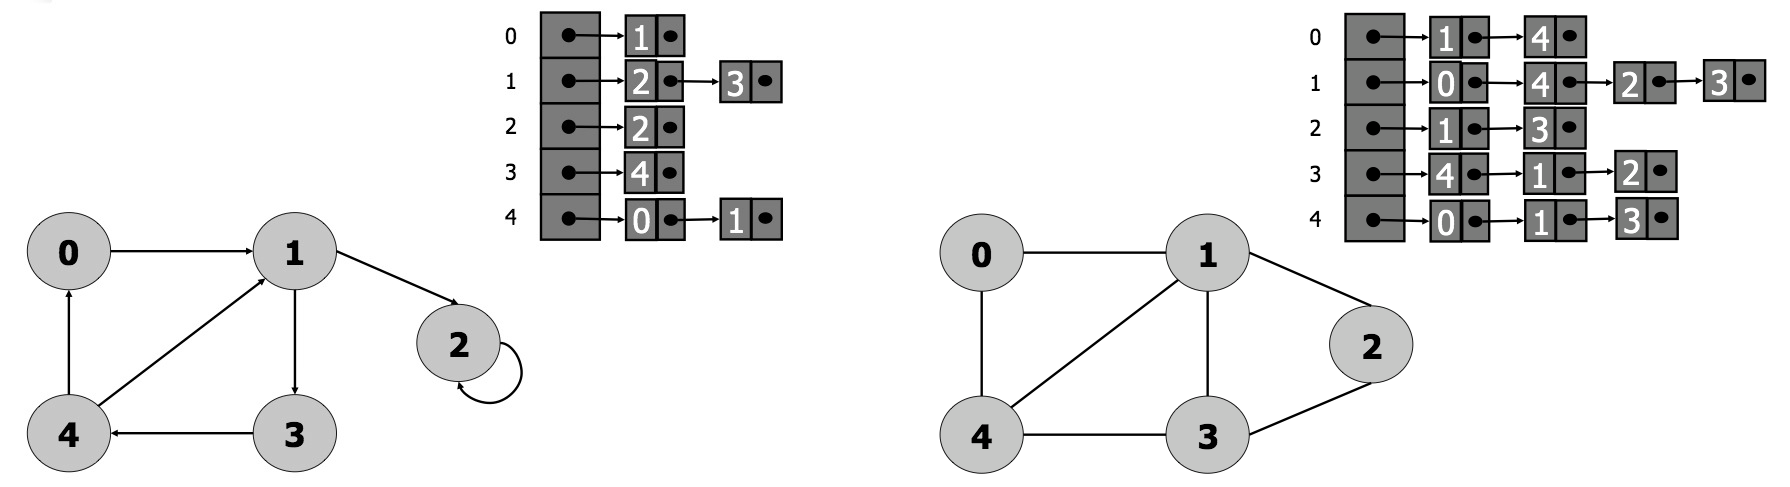
\includegraphics[angle=0,width=1\textwidth]{lists}
\end{center}
\caption{Rappresentazione con liste di adiacenza con grafi orientati (sinistra) e non orientati (destra)}
\end{figure}

La quantit\`a di memoria richiesta con questa tecnica di rappresentazione \`e $\Theta(V+E)$. La rappresentazione con liste di adiacenza \`e una soluzione molto compatta nel caso di grafi sparsi ed \`e anche molto robusta, cio\`e supporta molte varianti di grafi con minime modifiche; ad esempio, per i grafi pesati \`e sufficiente memorizzare il peso $w(u,v)$ assieme al vertice $v$ nella lista di adiacenza di $u$. 

Un possibile svantaggio di questo metodo riguarda l'impossibilit\`a di determinare in modo efficiente se un certo arco $(u,v)$ \`e presente nel grafo: tale analisi necessita la scansione della lista di adiacenza $A[u]$. Da questo punto di vista assai migliore \`e la memorizzazione tramite matrice di adiacenza.

\subsection{Rappresentazione con matrice di adiacenza}

\begin{figure}[h]
\begin{center}
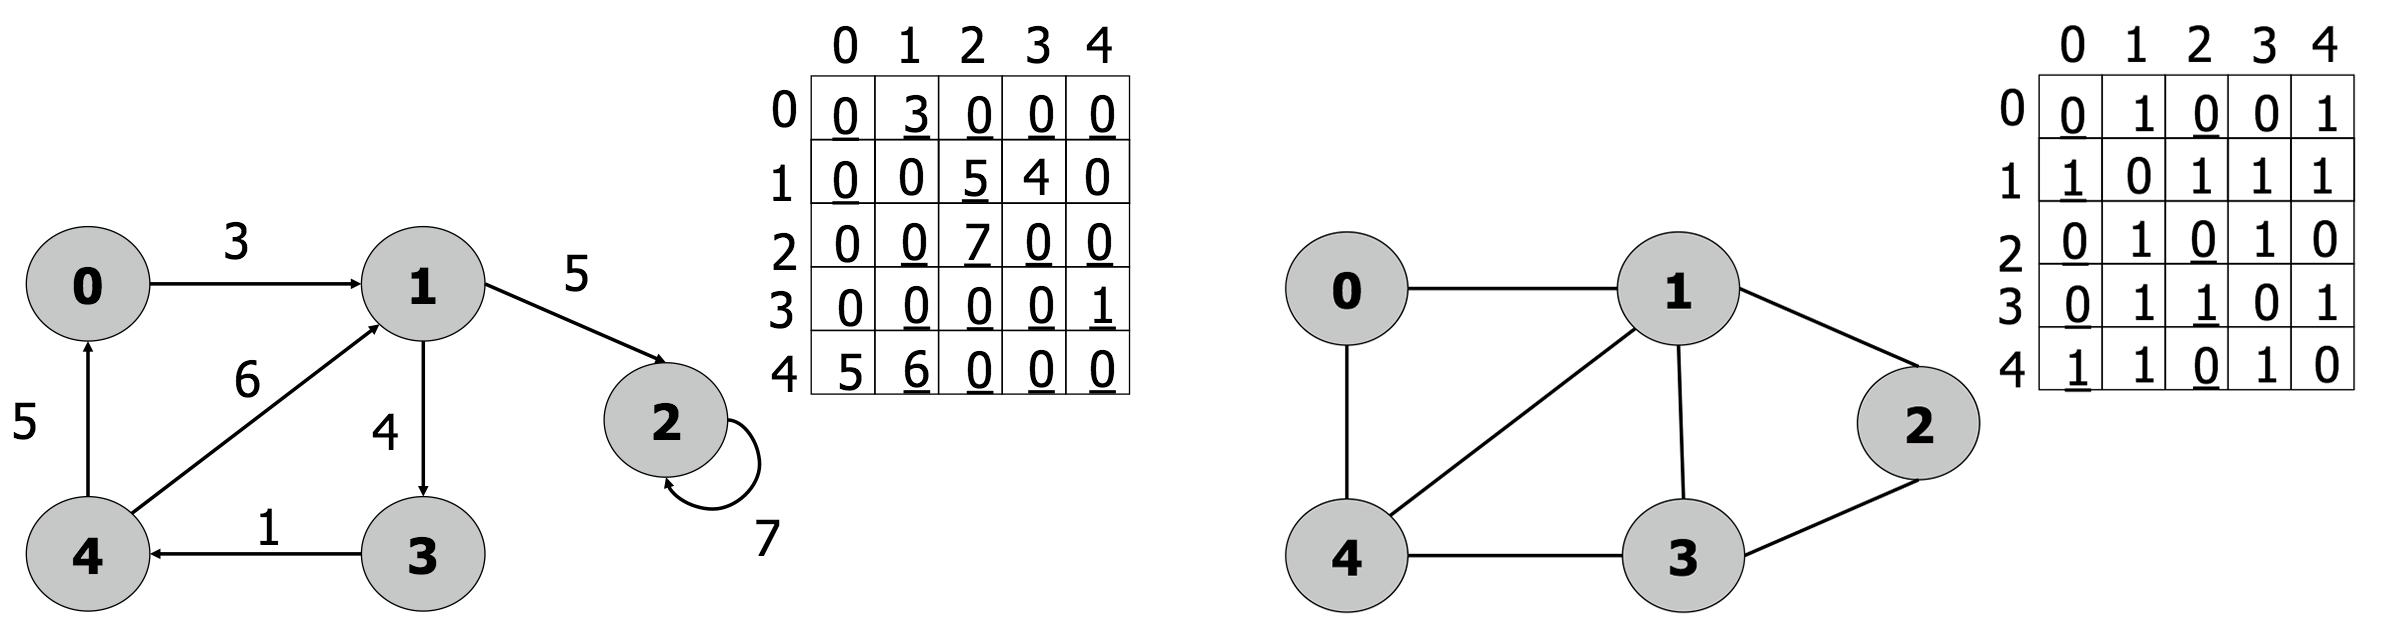
\includegraphics[angle=0,width=1\textwidth]{matrici}
\end{center}
\caption{Rappresentazione con matrici in caso di orientati pesati (sinistra) e grafi non orientati (destra)}
\end{figure}

Dato un grafo $G = (E,V)$, la rappresentazione con matrice di adiacenza fa uso di una matrice $M = (a_{ij})$ di dimensione $|V| \times |V|$. Tutti i vertici del grafo sono numerati in modo arbitrario, e nel caso in cui esista l'arco $(i,j)$ viene contrassegnata la cella della matrice $a_{ij}$ mediante l'assegnazione del valore di flag 1. Se l'arco non \`e previsto nel grafo in questione, il valore 0 viene assegnato. Dunque, indipendentemente dal numero di archi, la memoria necessaria in questo caso \`e $\Theta(V^2)$. In prima approssimazione, la rappresentazione con matrice di adiacenza \`e una buona soluzione in caso di grafi densi. Un'ottimizzazione in termini di memoria occupata \`e possibile per i grafi non orientati: in questo caso la matrice risultante \`e sempre simmetrica rispetto alla diagonale principale ({\em Figura 5, destra}), ed \`e quindi possibile dimezzare i dati memorizzati senza perdita di informazione.

Questa tipologia di rappresentazione \`e anche ottima nel caso dei grafi pesati, in quanto per salvare il peso associato a un arco \`e sufficiente sostituire il flag 1 nella posizione corrispondente della matrice con il valore stesso del peso. Questa soluzione non aumenta la memoria richiesta come invece avviene nel caso dei grafi pesati rappresentati mediante liste di adiacenza, in cui un valore a parte deve essere aggiunto per ogni arco.

Infine \`e importante notare quanto la topologia del grafo sia molto pi\`u accessibile con il metodo delle matrici, in quanto per verificare l'esistenza di un arco \`e sufficiente controllare la posizione corrispondente nella matrice.

\section{Algoritmi di ricerca}

Eseguire un algoritmo di ricerca su un grafo \`e detto anche {\bf visitare} il grafo. Il primo passo di una visita consiste nella scelta di un nodo di partenza, la {\bf sorgente}, da cui si raggiungono gli altri nodi del grafo seguendo gli archi sotto determinate regole. Durante questo processo \`e possibile memorizzare certe informazioni sulla struttura e contenuto del grafo. Durante la visita i nodi vengono concettualmente divisi per colori, cos\`i da poter tenere traccia del lavoro svolto:
\begin{itemize}
\item
{\em Bianco}: il nodo non \`e ancora stato visitato (non \`e stato scoperto);
\item
{\em Grigio}: il nodo \`e stato scoperto (visitato per la prima volta) ma non ancora completato (non sono stati ancora ispezionati tutti gli archi connessi al nodo);
\item
{\em Nero}: il nodo \`e stato scoperto e completato (tutti gli archi connessi al nodo sono stati ispezionati)
\end{itemize}

Esistono due principal algoritmi di ricerca per i grafi, sia orientati che non orientati: {\em visita in profondi\`a} (depth-first search, DFS) e {\em visita in ampiezza} (breadth-first search, BFS).

\subsection{Visita in profondit\`a (DFS)}
Partendo da un nodo sorgente $s$ scelto in modo arbitrario tra quelli di un grafo $G$, la visita in profondi\`a tocca tutti i nodi raggiungibili da $s$. Successivamente, se vi sono altri nodi non ancora visitati, tra questi viene scelto un nuovo nodo sorgente e la ricerca prosegue. La visita termina quando tutti i nodi del grafo sono stati visitati (anche se inizialmente non tutti sono raggiungibili, come nel caso di un grafo non orientato con pi\`u componenti connesse).

L'algoritmo di visita in profondi\`a si pu\`o suddividere in due componenti: 
\begin{itemize}
\item
{\bf GRAPHsearch}: procedura in cui si visitano tutti i nodi di un grafo mediante un ciclo (non ricorsivo) finch\'e tutti i nodi non siano diventati neri. Se un nodo visitato $v$ \`e classificato come bianco viene richiamata la procedura ricorsiva {\em dfsR}.
\item
{\bf dfsR}: procedura ricorsiva di visita in profondit\`a a partire dal nodo sorgente $v$ passato dalla {\em GRAPHsearch}. Con la {\em dfsR} gli archi vengono ispezionati a partire dall'ultimo vertice scoperto che ha ancora archi non ispezionati che escono da esso. Quando tutti gli archi di un certo nodo $u$ sono stati ispezionati, si procede con l'ispezione degli archi del nodo dal quale $u$ era stato scoperto. {\em dfsR} termina quando tutti i nodi raggiungibili dal nodo sorgente sono stati completati (neri).
\end{itemize}

Durante la visita, per ogni nodo viene registrato il {\bf tempo di scoperta} (quando il nodo diventa grigio) e il {\bf tempo di completamento} (quando il nodo diventa nero): il {\em tempo} consiste in un contatore che viene incrementato ad ogni fase della visita e i due parametri vengono salvati usando due array i cui indici sono associati ai vari nodi del grafo.
\\
%Inserire la figura del procedimento DFS

La visita di un grafo $G$ costruisce anche una {\bf foresta DF} (depth-first), tale per cui per ogni sorgente identificata durante la visita del grafo si genera un nuovo albero DF contente tutti i nodi raggiungibili dalla suddetta sorgente (oltre che la sorgente stessa). I nodi dei vari alberi DF vengono aggiunti e posizionati a seconda di come procede la visita del grafo. A partire dalla foresta DF risultante \`e possibile classificare gli archi di un grafo in diverse tipologie, utili per ulteriori analisi sul grafo (per esempio un grafo orientato \`e aciclico se e soltanto se una visita in profondit\`a non genera "archi all'indietro"):
\begin{itemize}
\item
{\em Archi d'albero}: l'arco $(u,v)$  \`e un arco d'albero se $v$ viene scoperto la prima volta durante l'ispezione del suddetto arco.
\item
{\em Archi all'indietro}: sono quegli archi che in un albero DF connettono un nodo con un suo antenato. Anche i cappi, che possono presentarsi nei grafi orientati, sono considerati archi all'indietro.
\item
{\em Archi in avanti}: sono gli archi (diversi da quelli d'albero) che connettono un nodo di un albero DF con un suo discendente.
\item
{\em Archi trasversali}: tutti gli altri archi.
\end{itemize}

Tali classificazioni valgono sia per i grafi orientati che non orientati; tuttavia, occorre specificare che in una visita di un grafo non orientato non si presentano mai archi in avanti e trasversali.

\begin{figure}[h]
\begin{center}
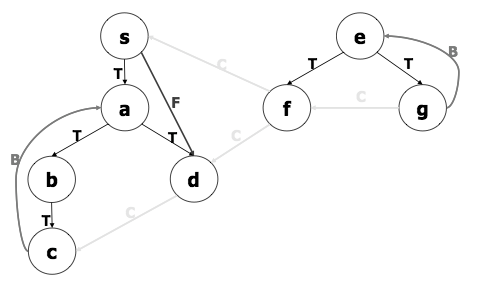
\includegraphics[angle=0,width=0.5\textwidth]{Archi}
\end{center}
\caption{Esempio di classificazione degli archi per un grafo orientato, con i nodi $s$ e $e$ selezionati come sorgenti per la visita: [T]: archi d'albero; [B] archi all'indietro; [F] archi in avanti; [C] archi trasversali}
\end{figure}

Per ci\`o che riguarda l'analisi di complessit\`a, questa pu\`o essere divisa per le due componenti dell'algoritmo: la parte del {\em GRAPHsearch} include un processo di inizializzazione che ha un costo per il quale si impiega un tempo $\Theta(|V|)$. La procedura {\em dfsR} viene invece invocata una volta per ogni arco del grafo: $\Theta(|E|)$. Se consideriamo l'adozione della rappresentazione del grafo con liste di adiacenza, il tempo di esecuzione della visita in profondit\`a \`e dunque: $\Theta(|V| + |E|)$. Una memorizzazione con matrice di adiacenza comporta un costo $\Theta(|V|^2)$.

\subsection{Visita in ampiezza (BFS)}
La visita in ampiezza ispeziona sistematicamente gli archi di un grafo G  per visitare tutti i nodi raggiungibili da un arbitrario nodo sergente $s$. Durante questo processo, l'algoritmo calcola il minimo numero di archi da $s$ a ciascun vertice raggiungibile, e salva l'informazione in un array i cui indici sono associati ai vari nodi del grafo. Inoltre viene generato un {\bf albero BF} (breadth-first) con radice $s$ e contenente tutti i nodi raggiungibili da $s$, memorizzati in modo che il cammino unico nell'albero BF che va da $s$ a $v$ corrisponde a un cammino minimo (percorso che contiene il minor numero di archi) da $s$ a $v$ nel grafo $G$.
 
L'algoritmo di visita in ampiezza necessita di una coda $Q$ con schema FIFO per gestire l'insieme dei nodi grigi mentre si procede con la visita. Inizialmente viene inserito nella coda l'elemento sorgente $s$ (a cui \`e associata una distanza 0 da $s$, se stesso). Successivamente l'algoritmo si ripete sempre allo stesso modo: 
\begin{itemize}
\item
Estrarre un elemento $v$ dalla coda. Il nodo diventa nero;
\item
Accodare tutti i nodi bianchi adiacenti al nodo $v$ precedentemente estratto. Questi nodi diventano grigi e ad essi viene associato il valore di distanza minima da $s$, uguale allo stesso valore assegnato a $v$ e incrementato di una unit\`a) ;
\item
Ripetere fino a quando non vi sono pi\`u elementi da poter estrarre dalla coda.
\end{itemize}

A seconda dell'ordine con cui vengono accodati i nodi bianchi adiacenti ad un certo nodo, l'albero BF risultante pu\`o variare leggermente, ma rimangono invariate le distanze calcolate dall'algoritmo per ognuno dei nodi del grafo.

%inserire la figura del procedimento BFS

Il tempo di esecuzione totale di BFS, come per il procedimento DFS, dipende da come il grafo \`e memorizzato nella memoria: nel caso di matrici di adiacenza, $T(n)=\Theta(|V|^2)$; nel caso di rappresentazione con liste di adiacenza: $T(n)=O(|V| + |E|)$.

\section{Applicazioni degli algoritmi di ricerca}
In questo paragrafo vengono brevemente presentati alcuni esempi di come gli algoritmi di ricerca trattati possano essere utilizzati per ricavare informazioni sulla struttura di un grafo.

\subsection{Identificazione di cicli}
Un grafo \`e aciclico se e solo se in seguito ad una visita in profondit\`a DFS non viene marcato alcun arco come "arco all'indietro".

\subsection{Componenti connessi}
Per un grafo non orientato ogni albero della foresta DF corrisponde a una componente connessa del grafo.

\subsection{Connettivit\`a}
Dato un grafo non orientato e connesso \`e possibile identificare i nodi o gli archi la cui rimozione comporterebbe la disconnessione del grafo. In questo caso si parla di {\bf ponte} per gli archi e di {\bf punto di articolazione} per i nodi. 

Un arco marcato come "arco all'indietro" non pu\`o essere un ponte. Un "arco d'albero" $(u,v)$ \`e un ponte se e solo se non ci sono altri "archi all'indietro" che connettono un discendente di $v$ con un antenato di $u$ nell'albero DF.

Se la radice dell'albero DF ha almeno due figli allora \`e un punto di articolazione del grafo. Qualsiasi altro nodo $v$ \`e un punto di articolazione se e solo se $v$ ha un figlio $u$ tale per cui non vi \`e alcun "arco all'indietro" da $u$ o da uno dei suoi discendenti a un antenato proprio di $v$.

\subsection{Ordinamento topologico}
L'ordinamento topologico di un grafico orientato aciclico, o {\em dag} (dall'inglese {\em directed acyclic graph}), \`e un ordinamento lineare di tutti i suoi vertici tale che per ogni arco $(u,v)$, $u$ appare prima di $v$ nell'ordinamento. Tale ordinamento si pu\`o intendere come una disposizione dei vertici di un {\em dag} lungo una linea orizzontale in modo che tutti gli archi del grafo (orientati) siano diretti da sinistra a destra. Questo procedimento pu\`o essere usato in molte applicazioni per modellare precedenze fra gli eventi.  

L'ordinamento topologico di un {\em dag} pu\`o essere ottenuto mediante una visita in profondit\`a del grafo: i tempi di completamento ottenuti dalla visita rappresentano l'ordine con cui disporre i nodi in modo da ottenere un orientamento topologico inverso, per il quale gli archi sono orientati da destra verso sinistra e per ogni arco $(u,v)$ il nodo $u$ appare alla destra del nodo $v$.

\subsection{Componenti fortemente connesse}
\`E possibile identificare le componenti fortemente connesse di un grafo orientato mediante l'algoritmo di Kosaraju, che fa uso della procedura di visita in profondit\`a. L'algoritmo prevede i seguenti passaggi:
\begin{itemize}
\item
Ottenere il grafo trasposto di $G$, $G$\textsuperscript{T}. Dato il grafo $G=(V,E)$, il trasposto $G$\textsuperscript{T}=$(V,E$\textsuperscript{T}$)$ \`e tale per cui per ogni arco $(u,v) \in E$ esiste l'arco $(v,u)$ in $E$\textsuperscript{T}.
\item
Eseguire DFS su $G$\textsuperscript{T}, ottenendo i tempi di scoperta e tempi di completamento di ogni nodo.
\item
Eseguire una nuova DFS sul grafo $G$ originale, facendo s\`i che nel ciclo principale in {\em GRAPHsearch} i vertici vengano considerati in ordine decrescente rispetto ai tempi di completamento calcolati dalla DFS del punto precedente.
\item
Gli alberi della foresta DF generata nel punto precedente corrispondono alle componenti fortemente connesse del grafo $G$.
\end{itemize}

\section{Alberi di connessione minimi (MST)}
Dato un grafo connesso e non orientato $G=(V,E)$, in cui a ogni arco $(u,v) \in E$ \`e associato un peso $w(u,v)$, un {\em albero di connessione minimo} (o "MST", dall'inglese {\em minmum spanning tree}) corrisponde ad un sottoinsieme aciclico $T \subseteq E$ che collega tutti i vertici in $V$ e il cui peso totale (la somma dei pesi dei singoli archi) sia minimo. Per un certo grafo possono esistere molteplici alberi di connessione minimi.

\begin{figure}[h]
\begin{center}
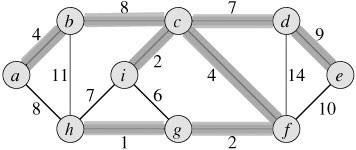
\includegraphics[angle=0,width=0.5\textwidth]{mst}
\end{center}
\caption{Gli archi evidenziati rappresentano un albero di connessione minimo per il grafo connesso d'esempio}
\end{figure}

Due algoritmi permettono di identificare alberi di connessione minimi: l'algoritmo di {\bf Kruskal} e l'algoritmo di {\bf Prim}. Entrambi gli algoritmi sono {\em algoritmi golosi}. In generale un algoritmo goloso, basato sul fare le scelte che sembrano migliori in un particolare momento, non garantisce la soluzione globale ottimale. Tuttavia pu\`o essere dimostrato che i due algoritmi succitati, dato un grafo (connesso, non orientato e pesato) forniscono sempre l'albero di connessione minimo.
\\

Sia Kruskal che Prim sono due algoritmi che si basano sul seguente {\bf algoritmo generico}: dato un grafo $G=(V,E)$ come descritto in precedenza, viene definito un sottoinsieme $A$, inizialmente vuoto, degli archi in $E$; ad $A$ viene aggiunto uno alla volta un arco, detto {\bf arco sicuro}, tale per cui il sottoinsieme $A$ rappresenti ancora un sottoinsieme di qualche albero di connessione minimo. Tale processo iterativo termina quando gli archi in $A$ raggiungono tutti i vertici del grafo, e l'albero di connessione minimo \`e stato costruito.

L'intero problema per gli MST si riduce quindi all'identificazione, per ogni iterazione, di un arco sicuro. Per affrontare il problema \`e necessario introdurre alcune definizioni:

\begin{itemize}
\item
Dato un grafo non orientato $G=(V,E)$, un {\bf taglio} \`e una partizione di $V$ in $S$ e $V-S$. Dunque l'insieme dei vertici $V$ \`e uguale a: $V \cup (V-S)$. Inoltre, $S \cap (V-S) = \oslash$.
\item
Si dice che un arco $(u,v) \in E$ {\bf attraversa} un taglio $(S,V-S)$ se uno dei due vertici $u$ e $v$ si trova in $S$ e l'altro in $V-S$.
\item
Un taglio {\bf rispetta} un insieme $A$ di archi se nessun arco dell'insieme $A$ attraversa il taglio.
\item
Un arco che attraversa un taglio \`e definito {\bf arco leggero} se il suo peso \`e minimo fra i pesi degli archi che attraversano il taglio stesso.
\end{itemize}

Partendo dalle precedenti definizioni \`e possibile introdurre il {\bf teorema degli archi sicuri}: dato un grafo $G=(V,E)$ (connesso, non orientato e pesato), si definisce $A$ come in sottoinsieme di $E$, nonch\'e un sottoinsieme di un qualche albero di connessione minimo per $G$; se possiamo identificare un taglio qualsiasi di $G$ che rispetta $A$ e un {\em arco leggero} che lo attraversa, allora quell'arco \`e sicuro per $A$.

Un {\bf corollario} del teorema degli archi sicuri stabilisce che, dato un grafo $G$ come descritto in precedenza e lo stesso sottoinsieme $A$ contenuto in qualche albero di connessione minimo per $G$, viene chiamata $C=(V_C,E_C)$ una componente connessa (un albero) della foresta $G_A=(V,A)$; un {\em arco leggero} che collega $C$ con qualche altra componente in $G_A$ \`e un arco sicuro per $A$.
\\

\subsection{Algoritmo di Kruskal}
L'algoritmo di Kruskal, basato sull'algoritmo generico descritto precedentemente, adotta il corollario del teorema degli archi sicuri per selezionare ad ogni iterazione un arco sicuro e costruire cos\`i l'albero di connessione minimo. 

In questo algoritmo l'insieme $A$ forma una foresta $G_A=(V,A)$, i cui alberi inizialmente corrispondono ai singoli vertici del grafo $G$ (in quanto inizialmente l'insieme $A$ \`e vuoto). Ad ogni iterazione dell'algoritmo generico viene selezionato un arco sicuro da aggiungere ad $A$, cio\`e un arco di peso minimo che collega due alberi qualsiasi della foresta $G_A$. Da questo procedimento si evince il motivo per il quale l'algoritmo di Kruskal rientra nella categoria degli algoritmi golosi: ad ogni passaggio si aggiunge alla foresta un arco con il minor peso possibile in quel momento. Le successive connessioni terminano al raggiungimento di un unico albero che contiene tutti i vertici del grafo iniziale.
\\
%inserire la figura dell'algoritmo di Kruskal

Il tempo di esecuzione dell'algoritmo di Kruskal dipende dall'implementazione della struttura dati. Adottando un'implementazione efficiente \`e possibile raggiungere un complessit\`a $T(n)=O(|E|lg|E|)$.

\subsection{Algoritmo di Prim}
Come per l'algoritmo di Kruskal, anche l'algoritmo di Prim si basa sull'algoritmo generico degli alberi di connessione minimi, ma in questo caso viene adottato il teorema degli archi sicuri (e non il suo corollario) per identificare, ad ogni iterazione, un arco sicuro.

Con l'algoritmo di Prim gli archi nell'insieme $A$ formano sempre un singolo albero, che inizia da un arbitrario vertice del grafo per poi svilupparsi fino a coprire tutti i vertici in $V$. Un taglio divide i vertici raggiunti dagli archi in $A$ da quelli non ancora raggiunti. Ad ogni passaggio viene aggiunto ad $A$ un arco leggero che attraversa il taglio (arco sicuro); prima di ripetere l'operazione, il taglio viene modificato perch\'e il nuovo vertice raggiunto dall'albero formato dagli archi in $A$ venga inserito nel sottoinsieme opportuno di $V$. La procedura termina quando l'albero formato dagli archi in $A$ raggiunge tutti i vertici $V$, diventando cos\`i un albero di connessione minimo del grafo.
\\
%inserire la figura dell'algoritmo di Prim

Adottando strutture dati efficienti, l'analisi di complessit\`a dell'algoritmo di Prim produce il seguente risultato: $T(n)=O(|E| + |V| lg |V|))$.

\section{Cammini minimi da sorgente unica (SSSP)}
Il problema dei {\em cammini minimi da sorgente unica} (o "SSSP", dall'inglese {\em single source shortest paths}), si propone di ispezionare un grafo di partenza $G=(V,E)$, che sia {\bf orientato e pesato}, per trovare i cammini minimi che partendo da un arbitrario vertice sorgente $s \in V$ raggiungono ciascun vertice $v \in V$. In altre parole, per ogni vertice $v \in V$ si vuole trovare un cammino con peso minimo da $s$ a $v$. 

\begin{figure}[h]
\begin{center}
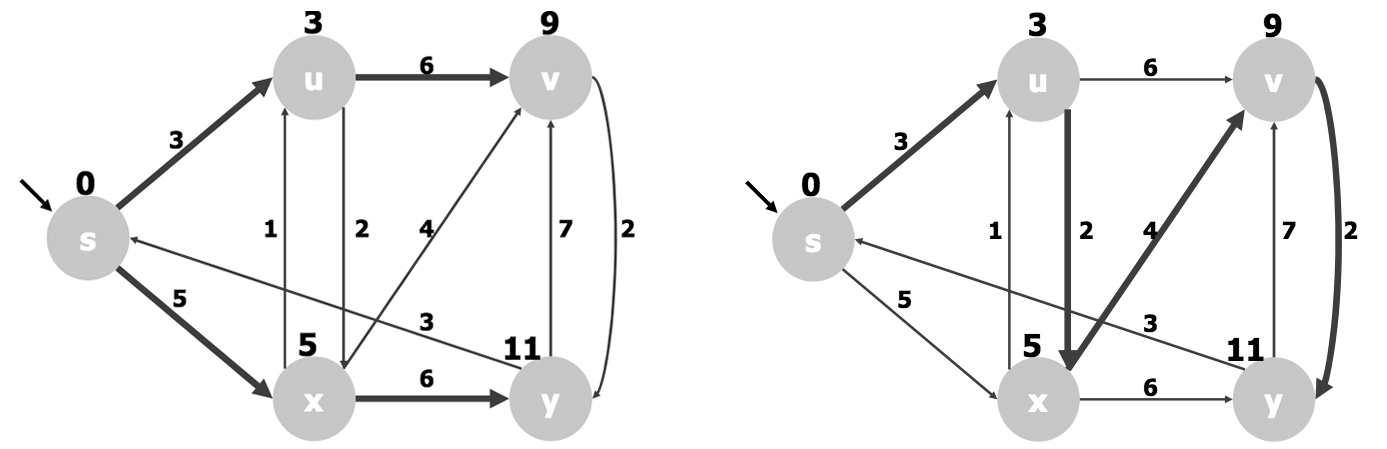
\includegraphics[angle=0,width=1\textwidth]{sssp}
\end{center}
\caption{Per il grafo orientato e pesato d'esempio, due possibili cammini minimi da sorgente $s$ sono indicati dagli archi pi\`u spessi. I valori evidenziati sopra i vari nodi indicano il peso del cammino minimo da $s$ per ciascun nodo}
\end{figure}

Il peso di un cammino \`e definito come la somma dei pesi degli archi che lo compongono; il peso di un arco $(u,v)$ viene indicato come $w(u,v)$. Il {\bf peso di un cammino minimo} tra due nodi $u$ e $v$ \`e pari al peso del cammino che \`e il minore tra tutti i pesi dei possibili cammini che connettono $u$ e $v$ oppure \`e infinito se non esiste un cammino tra $u$ e $v$. Un {\bf cammino minimo} tra i nodi $u$ e $v$ \`e dunque un qualsiasi cammino tra $u$ e $v$ il cui peso \`e uguale al peso minimo (molteplici cammini possono corrispondere alla descrizione, infatti cammini minimi tra due nodi non sono sempre unici).

Il concetto di {\bf peso} (o {\bf costo}) associato agli archi di un grafo pu\`o essere utile per modellare in generale qualsiasi quantit\`a penalizzante che si accumula linearmente lungo un cammino e che occorre minimizzare; ad esempio se il grafo \`e usato per modellare le connessioni stradali tra vari centri urbani, il costo degli archi pu\`o indicare la distanza tra le varie citt\`a.
\\

L'algoritmo che si sceglie di adoperare per identificare i cammini minimi da sorgente unica, pu\`o risolvere numerose varianti del problema, incluse le seguenti:

\begin{itemize}
\item
{\em Problema dei cammini minimi con destinazione unica}: trovare un cammino minimo da un ciascun vertice $v$ a un dato vertice destinazione $t$. Il problema \`e simmetrico a quello dei cammini minimi da sorgente unica;
\item
{\em Problema del cammino minimo per una coppia di vertici}: trovare un cammino minimo da $u$ a $v$, noti i vertici $u$ e $v$. La soluzione del problema dei cammini minimi da sorgente unica risolve anche questo problema;
\item
{\em Problema dei cammini minimi fra tutte le coppie di vertici}: trovare un cammino minimo da $u$ a $v$ per ogni coppia di vertici $u$ e $v$. Questo problema pu\`o essere risolto applicando l'algoritmo per sorgente unica una volta per ogni nodo del grafo di partenza, anche se esistono soluzioni pi\`u efficienti.
\end{itemize}

I due algoritmi proposti in questo capitolo per la soluzione del problema dei cammini minimi da sorgente unica sono l'algoritmo di {\bf Dijkstra} e l'algoritmo di {\bf Bellman-Ford}. I due algoritmi si comportano in modo differente in presenza di archi con peso negativo e cicli con peso negativo (cicli per i quali la somma dei pesi degli archi che li compongono sia negativa). 

Se esistono archi del grafo con peso negativo ma non esistono cicli negativi, l'algoritmo di Dijkstra non garantisce la soluzione ottimale al problema, mentre l'algoritmo di Bellman-Ford garantisce la soluzione ottimale.

Se esistono cicli con peso negativo {\bf non esiste una soluzione} al problema dei cammini minimi da sorgente unica: l'algoritmo di Dijkstra mostra un risultato senza valore, mentre l'algoritmo di Bellman-Ford \`e in grado di identificare i cicli negativi e non mostra alcun risultato.
\\

Nel contesto degli SSSP i cicli negativi non permettono di raggiungere un risultato valido in quanto i cammini verso i nodi facenti parte del ciclo (ed eventualmente altri nodi) risulterebbero avere un peso di cammino minimo negativo infinito; infatti \`e sempre possibile trovare un cammino di peso minore seguendo il ciclo di peso negativo. 

\begin{figure}[h]
\begin{center}
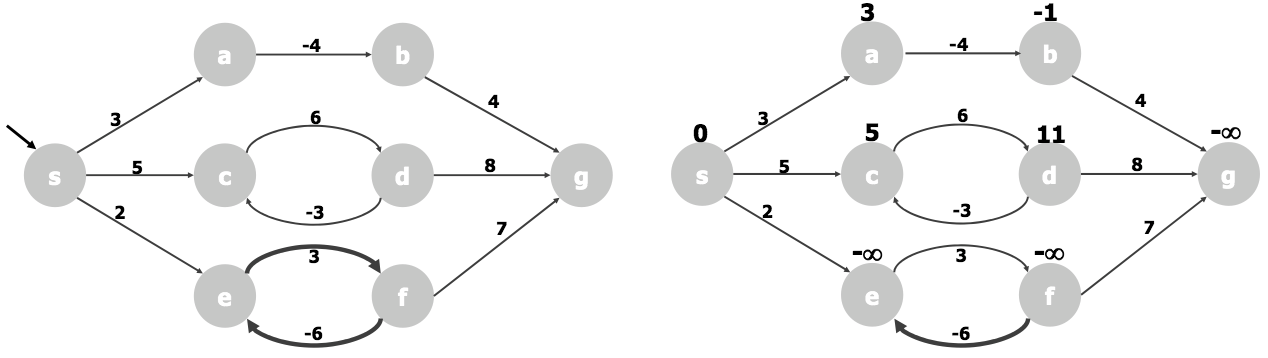
\includegraphics[angle=0,width=01\textwidth]{cicli}
\end{center}
\caption{Soluzione (senza valore) del problema dei cammini minimi da sorgente unica in caso di cicli negativi}
\end{figure}

Se si sceglie di rappresentare la soluzione del problema SSSP tramite un albero dei cammini minimi si pu\`o notare il forte legame con la procedura di visita in ampiezza di un grafo e l'albero BF risultante. Il problema dei cammini minimi per grafi non pesati \`e infatti risolubile adottando la procedura BFS.
\\

In relazione ai cammini minimi viene ora introdotto un importante lemma: i {\bf sottocammini di cammini minimi sono cammini minimi}. Per sottocammino si intende una porzione del cammino originario, tale da connettere due nodi qualsiasi $i$ e $j$ attraversati dal cammino originario. Il sottocammino sar\`a dunque un cammino minimo da $i$ a $j$. 

\`E possibile suddividere un cammino minimo $p$ tra i vertici $s$ e $v$ in due parti: un sottocammino da $s$ a $u$ e un arco $(u,v)$; seguendo il lemma precedente, il peso del cammino minimo tra $s$ e $v$ corrisponde al peso del cammino minimo tra $s$ e $u$ pi\`u il peso dell'arco $(u,v)$ ottenuto dalla suddivisione del cammino minimo originario. Dunque, per $\forall(u,v) \in E$, il cammino minimo tra $s$ e $v$ non pu\`o avere un peso maggiore del peso del cammino minimo da $s$ a $u$ sommato al peso di un arco $(u,v)$. 
\\

Gli algoritmi di Dijkstra e Bellman-Ford adottano la tecnica del {\bf rilassamento}. Dato un grafo $G=(V,E)$ come definito precedentemente (orientato e pesato), per ogni nodo $v \in V$ manteniamo un attributo $wt[v]$ che chiamiamo {\em stima del cammino minimo} per quel dato nodo. Il processo di rilassamento di un arco $(u,v)$ consiste nel verificare se, passando per $u$, \`e possibile migliorare la stima del cammino minimo di $v$; in altre parole viene verificato se la somma $wt[u] + w(u,v)$ \`e minore del valore $wt[v]$. Se ci\`o \`e verificato viene aggiornata la stima del cammino minimo di $v$ con il valore $wt[u] + w(u,v)$, e gli algoritmi di Dijkstra o Bellman-Ford registrano l'operazione per il raggiungimento del risultato finale (ottimale per tutti i nodi). Dopo il rilassamento di un arco $(u,v)$ o viene aggiornata (diminuita) la stima $wt[v]$ oppure non viene modificato nulla.

\begin{figure}[h]
\begin{center}
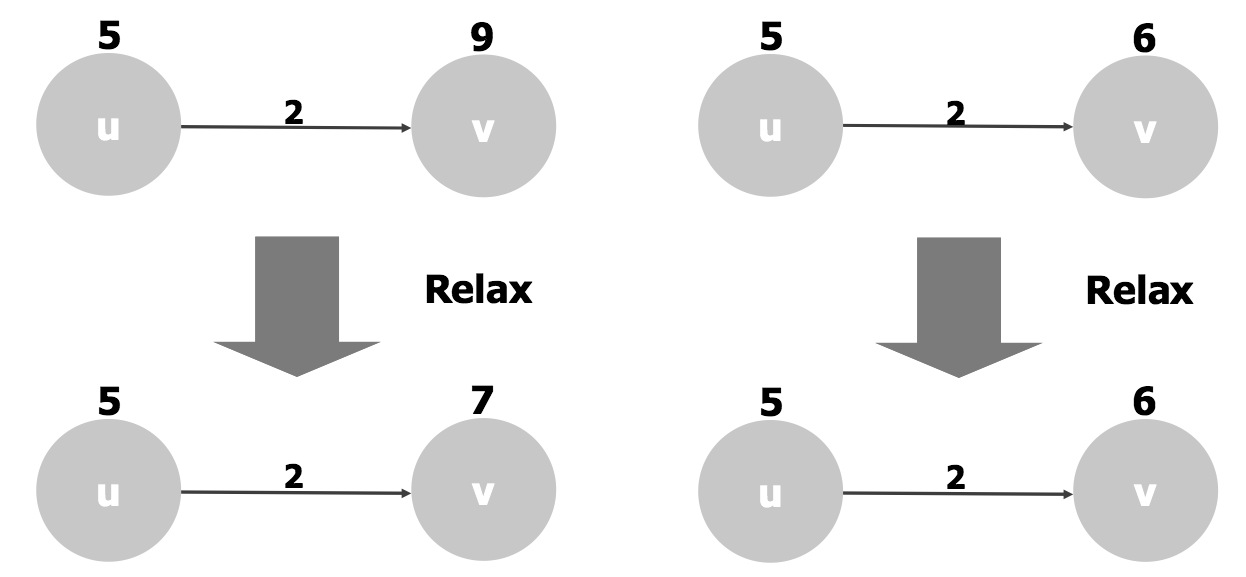
\includegraphics[angle=0,width=0.6\textwidth]{relax}
\end{center}
\caption{Due esempi di rilassamento di un arco $(u,v)$}
\end{figure}

Vengono ora proposti due ulteriori lemmi sul rilassamento, su cui sono basati gli algoritmi di Dijkstra e Bellman-Ford:
\begin{itemize}
\item
Quando $wt[v]$ corrisponde al peso del cammino minimo dalla sorgente $s$ al nodo $v$, non \`e pi\`u possibile ridurre $wt[v]$ tramite rilassamento.
\item
Quando un cammino minimo da $s$ a $v$ \`e scomponibile in un cammino minimo tra $s$ e $u$ e un arco $e=(u,v)$, se prima del rilassamento dell'arco $e$ la stima $wt[u]$ \`e uguale al peso del cammino minimo tra $s$ e $u$, dopo il rilassamento la stima $wt[v]$ \`e uguale al peso del cammino minimo tra $s$ e $v$.
\end{itemize}

Per l'ottenimento dei cammini minimi da sorgente unica, l'algoritmo di Dijkstra applica il rilassamento una volta per ogni arco del grafo, mentre lo stesso arco viene rilassato pi\`u volte con l'algoritmo di Bellman-Ford. 

\subsection{L'algoritmo di Dijkstra}
Per garantire la correttezza del risultato finale, l'algoritmo necessita che non siano presenti archi di peso negativo. I vertici del grafo di partenza vengono suddivisi in due sottoinsiemi: l'insieme $S$ dei nodi per i quali \`e stato compiuto il cammino minimo, e l'insieme $V-S$, i cui nodi (non ancora completati) sono inseriti in una coda min-prioritaria $Q$. Ad ogni iterazione dell'algoritmo viene estratto un nodo dalla coda per essere elaborato e aggiunto ad $S$. L'algoritmo termina quando la coda \`e vuota.

L'algoritmo prevede una prima fase di inizializzazione durante la quale la stima del cammino minimo del nodo scelto come sorgente $s$ \`e impostata a $0$ mentre la stima per tutti gli altri nodi \`e impostata ad un valore sufficientemente grande {\em maxWT}. Successivamente la coda viene riempita con tutti i nodi del grafo, seguendo una priorit\`a tanto maggiore quanto minore \`e la stima del cammino minimo.

Dopo la fase di inizializzazione inizia un processo iterativo per il quale ad ogni ciclo viene estratto dalla coda l'elemento $u$ avente il minimo valore di stima del cammino minimo $wt[u]$; tale elemento (che per la prima iterazione sar\`a il nodo sorgente), viene aggiunto all'insieme $S$ e per {\em ogni} vertice $v$ adiacente a $u$, viene rilassato l'arco $(u,v)$ (in altre parole, vengono rilassati tutti gli archi che escono da $u$).

La necessit\`a di scegliere, ad ogni iterazione, il vertice "pi\`u leggero" della coda $Q$ \`e il motivo per cui l'algoritmo di Dijkstra \`e definito come un algoritmo goloso, anche se \`e caratterizzato dalla propriet\`a non ordinaria di fornire sempre la soluzione globale corretta (se vengono rispettate certe condizioni sulle propriet\`a del grafo di partenza).
\\
%inserire la figura dell'algoritmo di Dijkstra

La complessit\`a dell'algoritmo di Dijkstra dipende dal metodo d'implementazione della coda di priorit\`a. Per l'analisi si possono studiare le operazioni critiche di cui l'algoritmo \`e composto. Se viene adottato un heap di Fibonacci per implementare la coda di priorit\`a, l'estrazione di un elemento ha un costo $O(lg|V|)$ e tale operazione \`e eseguita $|V|$ volte in quanto ogni nodo \`e estratto una sola volta. L'operazione di rilassamento richiede implicitamente delle operazioni di diminuzione di valore chiave per gli elementi della coda; tali operazioni vengono eseguite con un costo unitario nel caso dell'heap di Fibonacci. Il rilassamento \`e eseguito esattamente una volta per ogni arco in $E$. \`E dunque possibile ottenere un tempo di esecuzione pari a $O((|V|lg|V|)+|E|)$ se viene usato l'heap di Fibonacci per implementare la coda di priorit\`a.

\subsection{L'algoritmo di Bellman-Ford}
L'algoritmo consente la presenza di archi con peso negativo, ed \`e in grado di identificare i possibili cicli negativi presenti nel grafo; se almeno un ciclo negativo \`e presente, l'algoritmo indica che il problema non ha soluzione. 

La procedura Bellman-Ford necessita di una prima fase di inizializzazione delle stime dei cammini minimi simile a quella vista per l'algoritmo di Dijkstra: la stima di cammino minimo del nodo sorgente \`e impostata a $0$, mentre la stima degli altri nodi \`e impostata a {\em maxWT}. Successivamente \`e previsto un ciclo per cui ad ogni iterazione {\em tutti} gli archi in $E$ vengono rilassati senza un preciso ordine; tale ciclo viene eseguito un numero di volte pari al numero di vertici del grafo diminuito di uno, $|V|-1$. Al termine di questo processo viene eseguito il test per verificare la presenza di cicli negativi, che consiste in un ulteriore rilassamento per ogni arco: infatti, se al rilassamento $|V|$-esimo di uno degli archi viene migliorata una stima di cammino minimo, si pu\`o dimostrare che il grafo presenta almeno un ciclo negativo, e l'algoritmo non fornisce alcuna soluzione. 

L'algoritmo di Bellman-Ford necessit\`a di un numero di operazioni di rilassamento relativamente molto maggiore rispetto alla soluzione di Dijkstra. Tuttavia \`e possibile ottimizzare l'algoritmo in questione seguendo la regola per la quale se ad un qualsiasi ciclo {\em precedente} al ciclo $|V|$-esimo (di verifica) nessuna stima viene migliorata, la procedura pu\`o terminare garantendo che la soluzione ottimale \`e stata raggiunta.
\\
%inserire la figura dell'algoritmo di Bellman-Ford

L'algoritmo di Bellman-Ford prevede un'inizializzazione che richiede un tempo $\Theta(|V|)$, ciascuno dei $|V|-1$ cicli di rilassamento richiede un tempo $\Theta(|E|)$ e l'ultimo ciclo di verifica richiede un tempo $O(|E|)$. L'algoritmo viene dunque eseguito nel tempo $O(|V||E|)$.

\end{document}  